\begin{figure}[H]
    \centering

\begin{tikzpicture}
\pgfplotsset{
    every axis/.style={ymin=0},
    width=0.22\textwidth,
    height=0.25\textheight,
    xtick={2, 3, 4, 5, 6, 7, 8, 9, 10},
    y axis style/.style={
    yticklabel style=#1,
    ylabel style=#1,
    y axis line style=#1,
    ytick style=#1}}
\begin{axis}[ scale only axis, ymin=500, xmin=2,xmax=10, axis y line*=left, xlabel=Number of Cores, ylabel=Duration (s), y axis style=green!75!black]
    \addplot[smooth, green!75!black, mark=o, draw] 
    coordinates 
    {
        (2,747)
        (3,696)
        (4,676)
        (5,666)
        (6,656)
        (7,660)
        (8,656)
        (9,654)
        (10,654)
    };
\end{axis}
%
\begin{axis}[ scale only axis, ymin=4000, xmin=2,xmax=10, axis y line*=right, axis x line=none, ylabel=DEC (j), y axis style=blue]%
    \addplot[smooth, blue, mark=x] 
    coordinates 
    {
        (2,6746)
        (3,6457)
        (4,6371)
        (5,6314)
        (6,6319)
        (7,6260)
        (8,6319)
        (9,6227)
        (10,6224)
    };
\end{axis}
%
\begin{axis}[red, scale only axis, ymin=3, xmin=2,xmax=10, axis y line*=right, axis x line=none, ylabel=DEC per second (w)]%
\pgfplotsset{every outer y axis line/.style={xshift=2cm}, every tick/.style={xshift=2cm}, every y tick label/.style={xshift=2cm} }
    \addplot[smooth, red ,mark=+] 
    coordinates 
    {
        (2,4.477444127230992)
        (3,4.4619282394729884)
        (4,4.511881556635796)
        (5,4.512795211315868)
        (6,4.585327540101691)
        (7,4.444353491863994)
        (8,4.381832828098494)
        (9,4.219893166851358)
        (10,3.9391895804218375)
    };
\end{axis} 

\end{tikzpicture}
    \caption{The evolution of the DEC (blue), DEC per second (red) and duration (green) as more cores are allocated to PCM on DUT 2. Note that the x- and y- axis does not start at zero.}
    \label{fig:exp_3_dut_2_pcm_result}
\end{figure}